\begin{figure}[htpb]
	\centering\capstart{}
	\subfloat[\(\pixel{\Phi}\)]
	{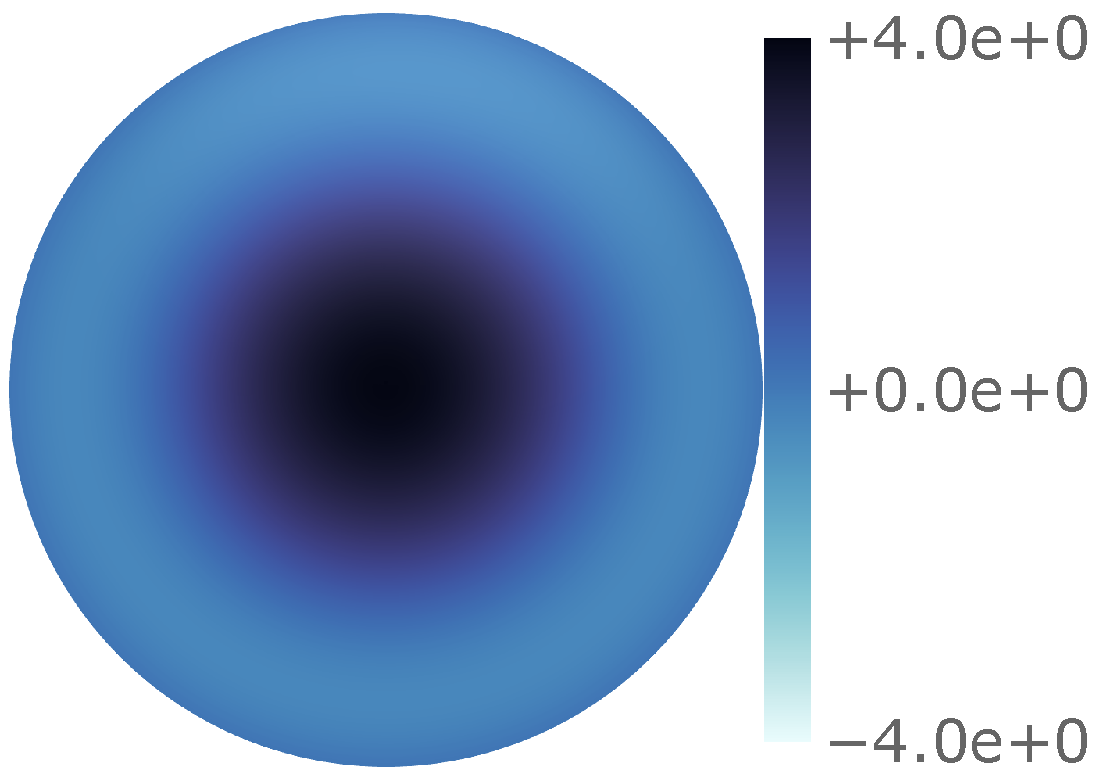
\includegraphics[trim={4 7 3 6},clip,width=.33\textwidth]{axisymmetric_wavelets_3B_2jmin_scaling_L128_res512_real.pdf}}
	\hfill
	\subfloat[\(\pixel{\Psi^{2j}}\)]
	{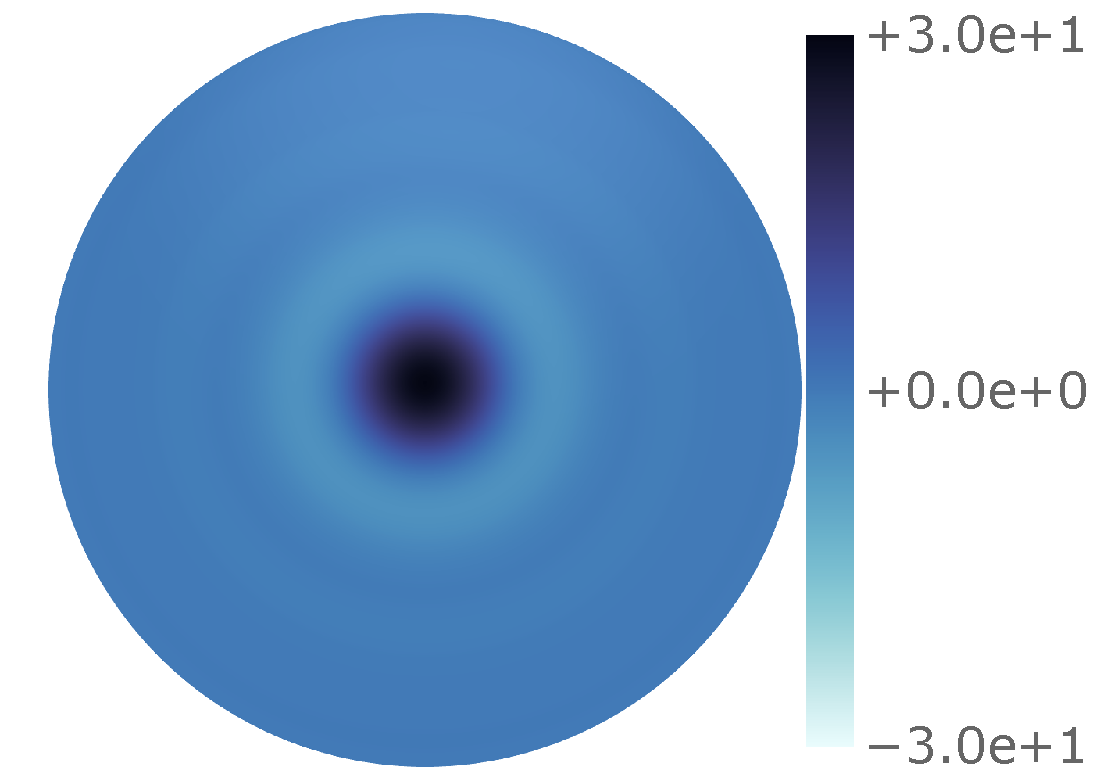
\includegraphics[trim={4 7 3 6},clip,width=.33\textwidth]{axisymmetric_wavelets_3B_2jmin_2j_L128_res512_real.pdf}}
	\hfill
	\subfloat[\(\pixel{\Psi^{3j}}\)]
	{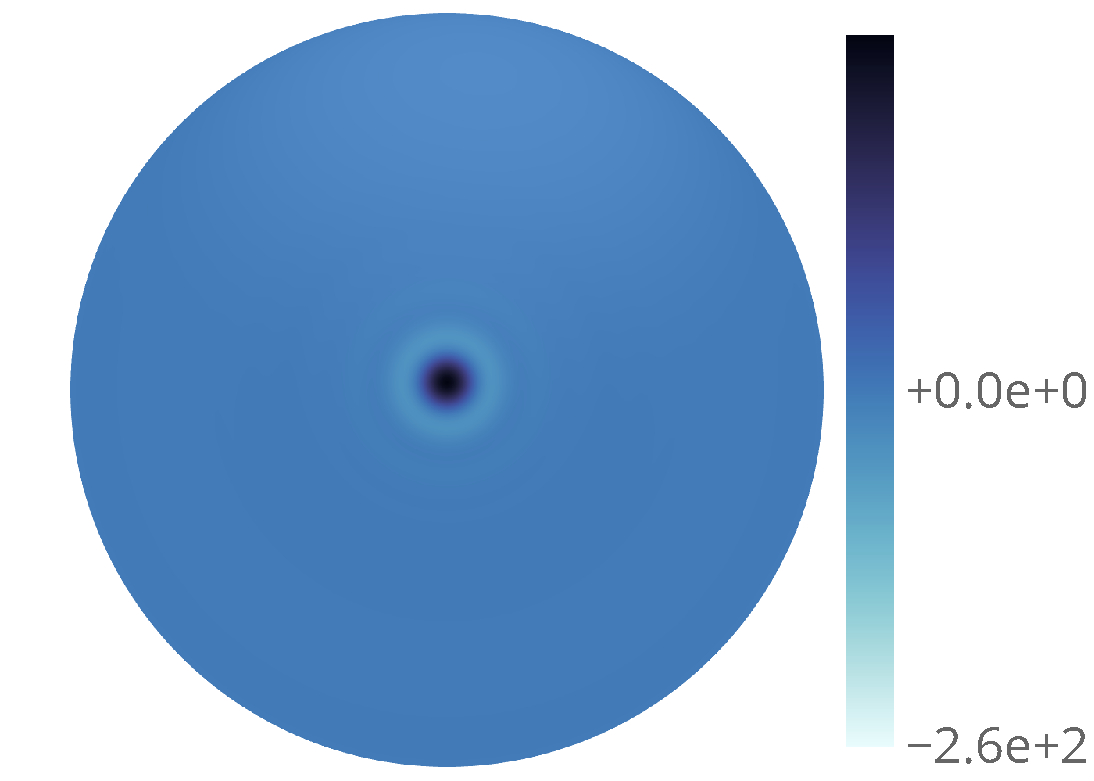
\includegraphics[trim={4 7 3 6},clip,width=.33\textwidth]{axisymmetric_wavelets_3B_2jmin_3j_L128_res512_real.pdf}}
	\newline
	\subfloat[\(\pixel{\Psi^{4j}}\)]
	{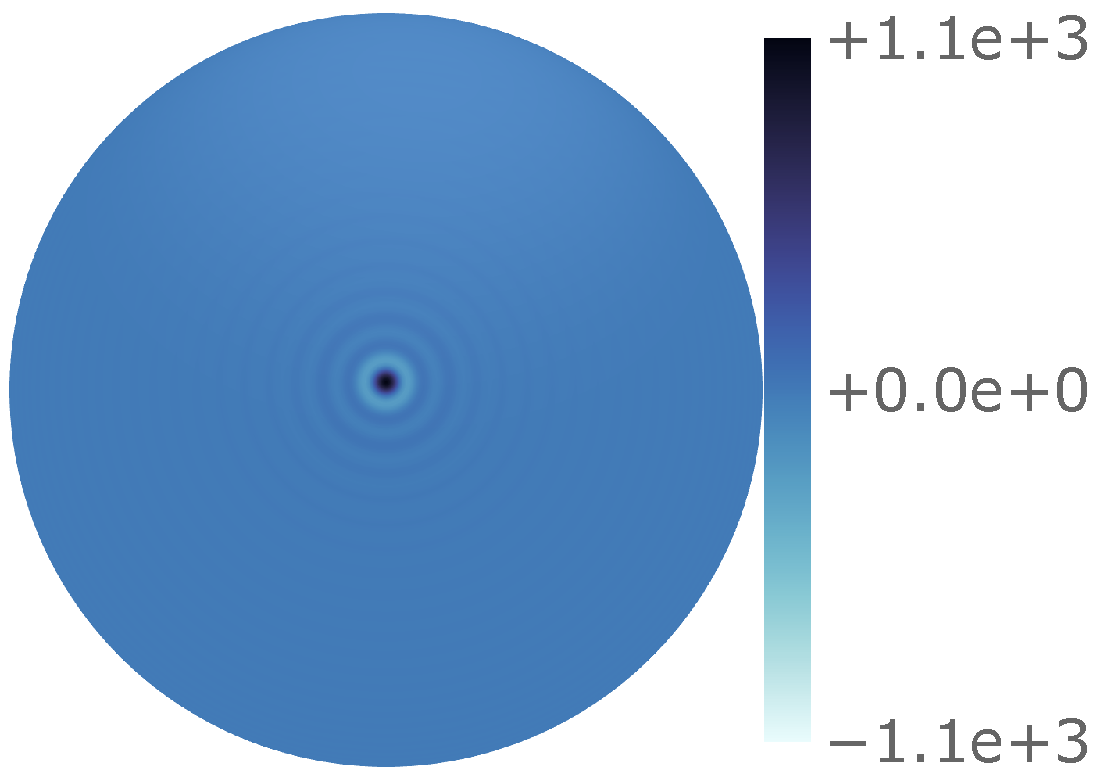
\includegraphics[trim={4 7 3 6},clip,width=.33\textwidth]{axisymmetric_wavelets_3B_2jmin_4j_L128_res512_real.pdf}}
	%
	\subfloat[\(\pixel{\Psi^{5j}}\)]
	{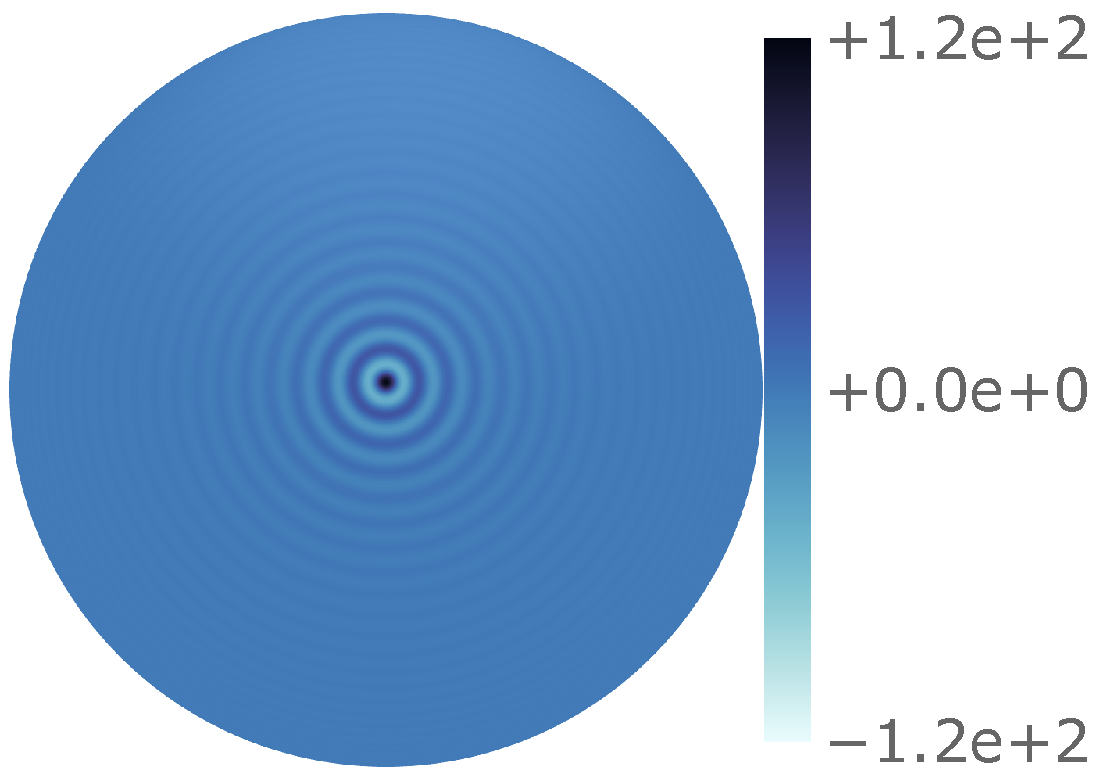
\includegraphics[trim={4 7 3 6},clip,width=.33\textwidth]{axisymmetric_wavelets_3B_2jmin_5j_L128_res512_real.pdf}}
	\caption[
		Some axisymmetric scale-discretised wavelets on the sphere
	]{
		The scaling function and the wavelets for scales \(j \in \set{2, 3, 4, 5}\) of the axisymmetric scale-discretised wavelets on the sphere centred on the north pole shown left-to-right, top-to-bottom.
		They are constructed through a tiling of the harmonic line with parameters \(\lambda=3\), \(J_{0}=2\), and bandlimit \(L=128\) (\cf{} \cref{fig:chapter2_tiling}).
	}\label{fig:chapter2_axisymmetric_wavelets}
\end{figure}
